\section{A three-dimensional, structured mesh example}
\label{sect:three_dimensional_example}
\par
The reader should be familiar with the geometry they will be creating in this section; the annulus
the reader opened and meshed in section \ref{ssect:basic_interaction_gmsh_gui} is the geometry
we will now create. The mesh however, will be of higher resolution. The following steps will be
undertaken, also outlined in figure \ref{fig:annulus_schematic}:
\begin{enumerate}
  \item Create the geometry using the Gmsh GUI:
  \begin{enumerate}
    \item A rectangle will be formed using a procedure similar to section
             \ref{sect:two_dimensional_example}. This rectangle represents a radial plane through the
             annulus, for example the plane outlined in red broken lines in the left panel of figure
             \ref{fig:annulus_schematic}.
    \item The plane will then be extruded-rotated in order to form a quadrant of the annulus, as
             shown in the right panel of figure \ref{fig:annulus_schematic}.
    \item The above step is then repeated, as indicated by the arrows in the top of the annulus on
             the left panel of figure \ref{fig:annulus_schematic}, until the complete annulus is formed
  \end{enumerate}
  \item Define physical groups.
  \item Customise the geometry by editing the geometry script file.
  \item Produce a mesh.
\end{enumerate}
\begin{figure}[htbp]
 \centering
  \includegraphics[width=1.0\textwidth]{../figures/annulus.pdf}
  \caption{Schematic of forming an annulus with extrusions}
  \label{fig:annulus_schematic}
\end{figure}

\subsection{Creating the geometry: Forming an annulus with extrusions}
\label{ssect:annulus_via_extrusions}
\par
Start Gmsh, at the command line using file \lstinline+annulus.geo+ to store the script. Create the three
points at the coordinates shown in table \ref{table:annulus_starting_points} below. The points should
lie on a line along the $x$-direction and form a radial line across the annulus. Create two lines: the
first line connecting point $1$ to point $2$ and the second
line connecting the point $2$ to point $3$. Then, extrude the lines to create surfaces
(extrude-translate, see figures \ref{fig:gmsh_extrusion} and \ref{fig:extrusion}), translating
by $(x,y,z)=(0.0, 0.0, 14.0)$. Note that both lines should be selected during the extrusion step.
Finally, change the view-point, so that you can see the rectangles just created, you should have
something similar to the graphic window in figure \ref{fig:extruding_red_plane}, corresponding to
the plane highlighted by the red broken line in the left panel of figure \ref{fig:annulus_schematic}
\begin{table}[htdp]
  \caption{Coordinates and mesh size at the starting points when making an annulus.}
  \centering
  \begin{tabular}{|r|c|c|c|c|}\hline
  point ID & $x$-coord. & $y$-coord. & $z$-coord. & Mesh element size \\ \hline
  $1$      & $2.5$      & $0.0$      & $0.0$      & $0.1$ \\ \hline
  $2$      & $5.25$     & $0.0$      & $0.0$      & $1.0$ \\ \hline
  $3$      & $8.0$      & $0.0$      & $0.0$      & $0.1$ \\ \hline
  \end{tabular}
  \label{table:annulus_starting_points}
\end{table}
\begin{figure}[htbp]
 \centering
  \includegraphics[width=1.0\textwidth]{../figures/shot17.png}
  \caption{The Graphic, Menu and Contextual Geometry Definitions windows during an 
                extrusion-via-revolution step.}
  \label{fig:extruding_red_plane}
\end{figure}
\par
The next step is to extrude-rotate the rectangular surface in order to create the annulus.
\begin{enumerate}
  \item Go to the top-most level of the Geometry module in the Gmsh menu window.
  \item Click on \lstinline+Elementary entities > Extrude > Rotate > Surface+. The
        Contextual Geometry Definitions window will appear, on the Rotation tab. Also the surfaces will
        now be highlighted on the graphic window, as shown in the graphic window of figure
        \ref{fig:extruding_red_plane}. The Contextual Geometry Definitions window is used to define
        the axis of revolution and the sweeping angle. The axis of revolution is defined by specifying any
        point on it and the components of a vector parallel to the axis. (\eg the red point and red vector
        components in the right panel of figure \ref{fig:annulus_schematic}). In addition, the sweeping angle
        must be specified in radians, in the anti-clockwise sense.
  \item Change the parameters in the Contextual Definitions window to the following:
  \begin{itemize}
    \item X coordinate of an axis point: $0$
    \item Y coordinate of an axis point: $0$
    \item Z coordinate of an axis point: $0$
    \item X component  of axis direction: $0$
    \item Y component  of axis direction: $0$
    \item Z component  of axis direction: $1$
    \item Angle in radians: Pi/$2$
  \end{itemize}
  \item Pick both surfaces on the graphic window and press ``e''. A quarter of the annulus should have been
        formed in the graphic window, as shown in left panel of figure \ref{fig:completing_the_annulus}. 
        Without changing the parameters in the Contextual Geometry Definitions
        window, pick the newly formed surfaces normal to the $x$-axis (surface demarcated in green in figure
        \ref{fig:annulus_schematic}) and press the ``e'' key, to form half the annulus. Repeat the
        procedure to form the complete annulus, shown in the right panel of figure
        \ref{fig:completing_the_annulus}. 
\end{enumerate}
\begin{figure}[htbp]
 \centering
  \includegraphics[width=1\textwidth]{../figures/completing_the_annulus.png}
  \caption{The Gmsh window showing a quadrant (left panel) and the complete annulus (right panel).}
  \label{fig:completing_the_annulus}
\end{figure}

\subsection{Physical groups}
\label{ssect:3d_physical_groups}
\par
As in the previous section physical surfaces and volumes must be specified, start by specifying physical
surfaces:
\begin{enumerate}
  \item Go to the top-most level of the Geometry module in the Gmsh menu window.
  \item Click on \lstinline+Physical groups > Add > Surface+. Select the $8$ surfaces comprising the
        top of the annulus and press ``e''. Obviously you can pan, zoom and change your viewpoint
        to make selection easier. Press ``u'' to undo your last selection as hinted on the graphic
        window, if a wrong choice is made.
  \item Repeat for the bottom of the annulus, the inner wall, and the outer wall (in that order).
  \item Press ``q'' to abort the selection mode and end the command.
\end{enumerate}
Then specify physical volumes:
\begin{enumerate}
  \item Click on \lstinline+Volume+, on the Gmsh menu window. Volumes created by extrusions will
           be indicated by yellow spherical markers, one per volume entity.
  \item Pick all of the spherical markers. Once picked, a volume marker is highlighted in red.
  \item Press ``e'' to end the selection.
\end{enumerate}

\subsection{Final customisation of the script and mesh production}
\label{ssect:3d_geo_fine_tuning}
\par
At this point, a mesh can be produced, suitable for Fluidity simulations. The mesh will be unstructured
and it is left as an exercise to the reader to mesh the geometry. Should you choose to mesh the geometry at
this point, then once finished you must go to the top-most level of the Geometry module and click on
\lstinline+Reload+ to re-join us for this tutorial. The script is now modified to make Gmsh produce a
structured mesh:
\begin{enumerate}
  \item Open the script in a text editor.
  \item The script should be \emph{similar} to the first listing below.
  \item Edit the script to make it similar to the second listing below, and save it. You only
        have to append the \lstinline+Layers{};+ statements and insert the comments.
  \item Go to the top-most level of the Geometry module in the Gmsh menu window. and click
        \lstinline+Reload+.
\end{enumerate}
\lstinline+annulus.geo+ file as produced by
GUI.
\lstset{numbers=left}
\begin{lstlisting}
Point(1) = {2.5, 0, 0, 0.1};
Point(2) = {5.25, 0, 0, 1.0};
Point(3) = {8, 0, 0, 0.1};
Line(1) = {1, 2};
Line(2) = {2, 3};
Extrude {0, 0, 14} {
  Line{1, 2};
}
Extrude {{0, 0, 1}, {0, 0, 0}, Pi/2} {
  Surface{6, 10};
}
Extrude {{0, 0, 1}, {0, 0, 0}, Pi/2} {
  Surface{32, 54};
}
Extrude {{0, 0, 1}, {0, 0, 0}, Pi/2} {
  Surface{98, 76};
}
Extrude {{0, 0, 1}, {0, 0, 0}, Pi/2} {
  Surface{120, 142};
}
Physical Surface(185) = {93, 49, 159, 115, 71, 27, 180, 137};
Physical Surface(186) = {107, 151, 41, 85, 63, 19, 172, 129};
Physical Surface(187) = {141, 184, 31, 75};
Physical Surface(188) = {89, 111, 155, 45};
Physical Volume(189) = {4, 3, 1, 2, 8, 7, 5, 6};
\end{lstlisting}
\lstset{numbers=none}
\lstinline+annulus.geo+ script after editing.
\lstset{numbers=left}
\begin{lstlisting}
Point(1) = {2.5, 0, 0, 0.1};
Point(2) = {5.25, 0, 0, 1.0};
Point(3) = {8, 0, 0, 0.1};
Line(1) = {1, 2};
Line(2) = {2, 3};
Extrude {0, 0, 14} {
  Line{1, 2};Layers{25};
}
Extrude {{0, 0, 1}, {0, 0, 0}, Pi/2} {
  Surface{6, 10};Layers{30};
}
Extrude {{0, 0, 1}, {0, 0, 0}, Pi/2} {
  Surface{32, 54};Layers{30};
}
Extrude {{0, 0, 1}, {0, 0, 0}, Pi/2} {
  Surface{98, 76};Layers{30};
}
Extrude {{0, 0, 1}, {0, 0, 0}, Pi/2} {
  Surface{120, 142};Layers{30};
}
// Top
Physical Surface(185) = {93, 49, 159, 115, 71, 27, 180, 137};
// Bottom
Physical Surface(186) = {107, 151, 41, 85, 63, 19, 172, 129};
// Inner wall
Physical Surface(187) = {141, 184, 31, 75};
// Outer wall
Physical Surface(188) = {89, 111, 155, 45};
Physical Volume(189) = {4, 3, 1, 2, 8, 7, 5, 6};
\end{lstlisting}
\lstset{numbers=none}
\par
To mesh the annulus, go to the top-most level of the Mesh module and click ``3D'' on the Gmsh menu
window.Notice the gradation in cell size towards the wall, affected by a different characteristic mesh size in
Point $2$, see table \ref{table:annulus_starting_points} and the listings above.
